\documentclass[a4paper,10pt]{article}

\usepackage{url,parskip}%formatting
\usepackage{titlesec}
\usepackage{supertabular}
\usepackage[utf8]{inputenc}
\usepackage{graphicx}
\usepackage{wrapfig}

\usepackage{hyperref}

\usepackage{fullpage}

\titleformat{\section}{\large\scshape\raggedright}{}{0em}{}[\titlerule]
\titlespacing{\section}{0pt}{0pt}{0pt}

\begin{document}
\pagestyle{empty}
  \begin{wrapfigure}{r}{0.25\textwidth}
  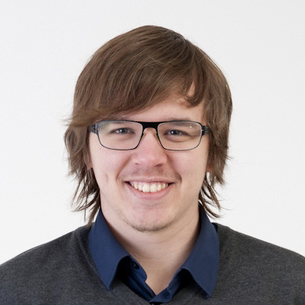
\includegraphics[width=0.25\textwidth]{fotogjengen_cropped.jpg}
  \end{wrapfigure}
% Title
\par{
  {\Huge Dag-Inge Aas }
  \bigskip\par}

% Personal Data
%  \section{Personal Data}
  \begin{tabular}{rl}
  \textsc{Date of Birth:} & 21 July 1989\\
    \textsc{Address:}& Sverresgate 8 B21, 7012 Trondheim\\
    \textsc{Phone:}& +47 924 91 526\\
    \textsc{Email:}& \href{mailto:daginge@gmail.com}{daginge@gmail.com}\\
    \textsc{Homepage:}& \href{http://daginge.com}{http://daginge.com}\\
    \textsc{Github:}& \href{http://github.com/dagingaa}{http://github.com/dagingaa}\\
\end{tabular}

\section{Summary}
\par{
Front-end developer with a passion for building tomorrow's applications and services for the web. Likes to do large scale system architecture and integration. Interested in new technologies, methodologies and hacking. }

\section{Education}
\begin{tabular}{r|p{12cm}}
  \textsc{Jun 2013} & \textsc{Norwegian University of Science and Technology} \\\textsc{Aug 2008}&\emph{Master of Science in Computer Science}\\&\footnotesize{Specialized in Software and Information Systems.} \\& \footnotesize{Notable courses: Object-oriented Programming, Algorithms and Data structures, Information Systems, Programming Languages, Software Architecture, Software Quality and Quality Assurance, Software Security, Distributed Systems, Project Management.}\\\multicolumn{2}{c}{} \\
\end{tabular}

\section{Work Experience}
\begin{tabular}{r|p{12cm}}
  \emph{Current} & Software Developer Intern at \textsc{Telenor Comoyo}, Trondheim \\\textsc{Jan 2012}&\emph{Software Development}\\&\footnotesize{Software developer. Currently working with scalable end-to-end browser testing in the cloud for Comoyo's services.

Full-time hire as a Summer Intern for Summer 2012.}\\\multicolumn{2}{c}{} \\
  \textsc{Jul 2011} & Summer Intern at \textsc{Iterate}, Oslo \\\textsc{Jun 2011}&\emph{IT consultancy}\\&\footnotesize{Developed a new customer-driven project in Java on Amazon Web Services. Learned about synchronization, REST and large-scale distributed systems and their issues. Personal coaching on SCRUM and Kanban by Iterate and Kent Beck. Arranged and held our own meetings. Norwegian attestation available on request.}\\\multicolumn{2}{c}{} \\
  \textsc{Jan 2012} & Guru at \textsc{Gurutjenesten}, NTNU  \\\textsc{Aug 2010}&\emph{First line IT-support}\\&\footnotesize{IT-support for the Department of Computer and Information Science (IDI) at NTNU. Customers include students and faculty members with tasks ranging from setup of hardware to debugging a faulty C compiler.}\\\multicolumn{2}{c}{} \\
  \textsc{Dec 2011} & Senior Teaching Assistant in TDT4110 Information Technology, NTNU  \\\textsc{Aug 2011}&\emph{Colloquium responsible}\\&\footnotesize{Help students fresh to programming understand the concepts of programming and the exercises given to them. Programming was mainly focused on Python and Matlab. Colloquiums are focused on helping students completely new to programming }\\\multicolumn{2}{c}{} \\
  \textsc{Dec 2009} & Teaching Assistant in TDT4110 Information Technology, NTNU  \\ \textsc{Aug 2009}&\emph{HTML, CSS, JSP and MySQL}\\\multicolumn{2}{c}{} \\
  \textsc{Aug 2010} & Customer advisor at \textsc{Expert}, Ålesund \\\textsc{Sep 2006}&\emph{Sales and customer support. Worked only holidays after 2008.}\\\multicolumn{2}{c}{} \\
\end{tabular}

\section{Volunteer work}
\begin{tabular}{r|p{12cm}}
  \emph{Current} & Head of IT at ISFiT 2013, Trondheim  \\\textsc{Aug 2011}&\emph{Head of Development and System Administration}\\&\footnotesize{The Head of IT is responsible for the entire infrastructure of ISFiT. This includes development, maintenance and system administration for a festival with over 400 volunteers. ISFiT has 5 major IT projects, ranging from editorial tools to system administration. I oversee the development and maintenance of these five projects, with 8 developers actively working on them. I also participate in board meetings in the information section, creating and spreading ISFiT 2013 to the world. See also "Head of Development"}\\\multicolumn{2}{c}{} \\
  \emph{Aug 2011} & Head of Development at ISFiT 2011, Trondheim  \\\textsc{Mar 2010}&\emph{Ruby on Rails Developer and Project Manager}\\&\footnotesize{Project manager for the biggest new IT project of ISFiT 2011. Held meetings, workshops and demonstrations, gathered requirement specification from the different affected parties and maintaned the project after launch. Led a group of 3 other developers from start to finish to maintenance. Programming was mainly focused on Ruby on Rails and scripting using Ruby. Some of our core technologies include LDAP, MySQL, UNIX, Apache, Passenger, capistrano and more.}\\\multicolumn{2}{c}{} \\
  \textsc{Aug 2011}& Excursion planner for \textsc{Xcom'11}, Trondheim \\\textsc{Jan 2010}& \emph{Excursion commitee}\\&\footnotesize{Responsible for the contact with the travel agency. Also did crisis management when the trip got cancelled due to an earthquake in Japan followed by a nuclear crisis.}\\\multicolumn{2}{c}{} \\
\end{tabular}

\section{Skills}
\begin{tabular}{r|p{12cm}}
  \textsc{Technical}& Programming languages  \\&\footnotesize{Java, Ruby, Javascript, Python. In addition the following frameworks and libraries: Ruby on Rails, Android, Amazon Web Services API. }
  \\&\par \\& Databases  \\&\footnotesize{MySQL, PostgreSQL, Amazon SimpleDB}
  \\&\par \\& Other  \\&\footnotesize{HTML(5), CSS(3), Amazon Web Services, XMPP, Project Management, RESTful API in Java}
  \\\multicolumn{2}{c}{}\\
  \textsc{Personal}& Languages  \\&\footnotesize{Norwegian (Native Language), English (Experienced), French (Written understanding)}

\end{tabular}

\section{References}
\begin{tabular}{rl}
  \textsc{Expert Norge} & Per-André Olsbø - 92808891 between 10 and 16 on weekdays
  \\& Jostein Brekke - 95888858 between 10 and 16 on weekdays
  \\\multicolumn{2}{c}{}\\
  \textsc{ISFiT}& Iver Dihle Skjervum - 99495245 on weekdays \\
\end{tabular}


\end{document}
